\documentclass[]{article}
\usepackage{lmodern}
\usepackage{amssymb,amsmath}
\usepackage{ifxetex,ifluatex}
\usepackage{fixltx2e} % provides \textsubscript
\ifnum 0\ifxetex 1\fi\ifluatex 1\fi=0 % if pdftex
  \usepackage[T1]{fontenc}
  \usepackage[utf8]{inputenc}
\else % if luatex or xelatex
  \ifxetex
    \usepackage{mathspec}
  \else
    \usepackage{fontspec}
  \fi
  \defaultfontfeatures{Ligatures=TeX,Scale=MatchLowercase}
\fi
% use upquote if available, for straight quotes in verbatim environments
\IfFileExists{upquote.sty}{\usepackage{upquote}}{}
% use microtype if available
\IfFileExists{microtype.sty}{%
\usepackage{microtype}
\UseMicrotypeSet[protrusion]{basicmath} % disable protrusion for tt fonts
}{}
\usepackage[margin=1in]{geometry}
\usepackage{hyperref}
\hypersetup{unicode=true,
            pdftitle={Regression: The Best Line},
            pdfborder={0 0 0},
            breaklinks=true}
\urlstyle{same}  % don't use monospace font for urls
\usepackage{color}
\usepackage{fancyvrb}
\newcommand{\VerbBar}{|}
\newcommand{\VERB}{\Verb[commandchars=\\\{\}]}
\DefineVerbatimEnvironment{Highlighting}{Verbatim}{commandchars=\\\{\}}
% Add ',fontsize=\small' for more characters per line
\usepackage{framed}
\definecolor{shadecolor}{RGB}{248,248,248}
\newenvironment{Shaded}{\begin{snugshade}}{\end{snugshade}}
\newcommand{\AlertTok}[1]{\textcolor[rgb]{0.94,0.16,0.16}{#1}}
\newcommand{\AnnotationTok}[1]{\textcolor[rgb]{0.56,0.35,0.01}{\textbf{\textit{#1}}}}
\newcommand{\AttributeTok}[1]{\textcolor[rgb]{0.77,0.63,0.00}{#1}}
\newcommand{\BaseNTok}[1]{\textcolor[rgb]{0.00,0.00,0.81}{#1}}
\newcommand{\BuiltInTok}[1]{#1}
\newcommand{\CharTok}[1]{\textcolor[rgb]{0.31,0.60,0.02}{#1}}
\newcommand{\CommentTok}[1]{\textcolor[rgb]{0.56,0.35,0.01}{\textit{#1}}}
\newcommand{\CommentVarTok}[1]{\textcolor[rgb]{0.56,0.35,0.01}{\textbf{\textit{#1}}}}
\newcommand{\ConstantTok}[1]{\textcolor[rgb]{0.00,0.00,0.00}{#1}}
\newcommand{\ControlFlowTok}[1]{\textcolor[rgb]{0.13,0.29,0.53}{\textbf{#1}}}
\newcommand{\DataTypeTok}[1]{\textcolor[rgb]{0.13,0.29,0.53}{#1}}
\newcommand{\DecValTok}[1]{\textcolor[rgb]{0.00,0.00,0.81}{#1}}
\newcommand{\DocumentationTok}[1]{\textcolor[rgb]{0.56,0.35,0.01}{\textbf{\textit{#1}}}}
\newcommand{\ErrorTok}[1]{\textcolor[rgb]{0.64,0.00,0.00}{\textbf{#1}}}
\newcommand{\ExtensionTok}[1]{#1}
\newcommand{\FloatTok}[1]{\textcolor[rgb]{0.00,0.00,0.81}{#1}}
\newcommand{\FunctionTok}[1]{\textcolor[rgb]{0.00,0.00,0.00}{#1}}
\newcommand{\ImportTok}[1]{#1}
\newcommand{\InformationTok}[1]{\textcolor[rgb]{0.56,0.35,0.01}{\textbf{\textit{#1}}}}
\newcommand{\KeywordTok}[1]{\textcolor[rgb]{0.13,0.29,0.53}{\textbf{#1}}}
\newcommand{\NormalTok}[1]{#1}
\newcommand{\OperatorTok}[1]{\textcolor[rgb]{0.81,0.36,0.00}{\textbf{#1}}}
\newcommand{\OtherTok}[1]{\textcolor[rgb]{0.56,0.35,0.01}{#1}}
\newcommand{\PreprocessorTok}[1]{\textcolor[rgb]{0.56,0.35,0.01}{\textit{#1}}}
\newcommand{\RegionMarkerTok}[1]{#1}
\newcommand{\SpecialCharTok}[1]{\textcolor[rgb]{0.00,0.00,0.00}{#1}}
\newcommand{\SpecialStringTok}[1]{\textcolor[rgb]{0.31,0.60,0.02}{#1}}
\newcommand{\StringTok}[1]{\textcolor[rgb]{0.31,0.60,0.02}{#1}}
\newcommand{\VariableTok}[1]{\textcolor[rgb]{0.00,0.00,0.00}{#1}}
\newcommand{\VerbatimStringTok}[1]{\textcolor[rgb]{0.31,0.60,0.02}{#1}}
\newcommand{\WarningTok}[1]{\textcolor[rgb]{0.56,0.35,0.01}{\textbf{\textit{#1}}}}
\usepackage{graphicx,grffile}
\makeatletter
\def\maxwidth{\ifdim\Gin@nat@width>\linewidth\linewidth\else\Gin@nat@width\fi}
\def\maxheight{\ifdim\Gin@nat@height>\textheight\textheight\else\Gin@nat@height\fi}
\makeatother
% Scale images if necessary, so that they will not overflow the page
% margins by default, and it is still possible to overwrite the defaults
% using explicit options in \includegraphics[width, height, ...]{}
\setkeys{Gin}{width=\maxwidth,height=\maxheight,keepaspectratio}
\IfFileExists{parskip.sty}{%
\usepackage{parskip}
}{% else
\setlength{\parindent}{0pt}
\setlength{\parskip}{6pt plus 2pt minus 1pt}
}
\setlength{\emergencystretch}{3em}  % prevent overfull lines
\providecommand{\tightlist}{%
  \setlength{\itemsep}{0pt}\setlength{\parskip}{0pt}}
\setcounter{secnumdepth}{0}
% Redefines (sub)paragraphs to behave more like sections
\ifx\paragraph\undefined\else
\let\oldparagraph\paragraph
\renewcommand{\paragraph}[1]{\oldparagraph{#1}\mbox{}}
\fi
\ifx\subparagraph\undefined\else
\let\oldsubparagraph\subparagraph
\renewcommand{\subparagraph}[1]{\oldsubparagraph{#1}\mbox{}}
\fi

%%% Use protect on footnotes to avoid problems with footnotes in titles
\let\rmarkdownfootnote\footnote%
\def\footnote{\protect\rmarkdownfootnote}

%%% Change title format to be more compact
\usepackage{titling}

% Create subtitle command for use in maketitle
\providecommand{\subtitle}[1]{
  \posttitle{
    \begin{center}\large#1\end{center}
    }
}

\setlength{\droptitle}{-2em}

  \title{Regression: The Best Line}
    \pretitle{\vspace{\droptitle}\centering\huge}
  \posttitle{\par}
  \subtitle{Ch. 5.2}
  \author{}
    \preauthor{}\postauthor{}
      \predate{\centering\large\emph}
  \postdate{\par}
    \date{Spring 2020}


\begin{document}
\maketitle

\hypertarget{the-setup}{%
\subsection{The Setup}\label{the-setup}}

\hypertarget{section}{%
\subsubsection{\texorpdfstring{\href{}{}}{}}\label{section}}

So you've identified two numeric variables that seem to have a moderate
to strong linear pattern. How can you find you find the best fitting
line? ``Eyeballing it'' just isn't going to cut it. We need a more
precise way.

\begin{itemize}
\item
  We can use the idea of \textbf{residuals} to quantify what ``best
  line'' means for modelling data.
\item
  Slope and intercept for the best line can easily be estimated using
  simple summary statistics (or R).
\item
  Predictions for new observations can then be made from our regression
  model.
\end{itemize}

\hypertarget{most-important}{%
\subsubsection{Most important}\label{most-important}}

We will be able to \textbf{interpret the slope coefficient} for our best
fitting linear regression equation. Why is this so important? Because we
don't want to lose sight of the original purpose of ANY statistical
analysis: defining patterns and relationships.

\begin{quote}
The slope of a linear regression line is a way to represent the
relationship between response and explanatory variables. It will be the
most important aspect of the regression model and what we focus on for
interpretation and inference.
\end{quote}

\hypertarget{a-note-about-conditions}{%
\subsubsection{A note about conditions}\label{a-note-about-conditions}}

There are conditions to using linear regression, some very familiar and
one new. The conditions are listed below, however, linear regression is
one of the few methods of analysis where it is easier to check the
conditions after the model has been found. So I will talk more about
these in the next tutorial.

\begin{itemize}
\item
  \textbf{Linearity}
\item
  \textbf{Nearly Normal residuals}
\item
  \textbf{Constant variance}
\item
  \textbf{Independent observations}
\end{itemize}

\hypertarget{least-squares-regression}{%
\subsection{Least Squares Regression}\label{least-squares-regression}}

\hypertarget{section-1}{%
\subsubsection{\texorpdfstring{\href{}{}}{}}\label{section-1}}

Recall from the last tutorial that \textbf{residuals} are the leftovers
from a model, the error between an observed and predicted value.

~

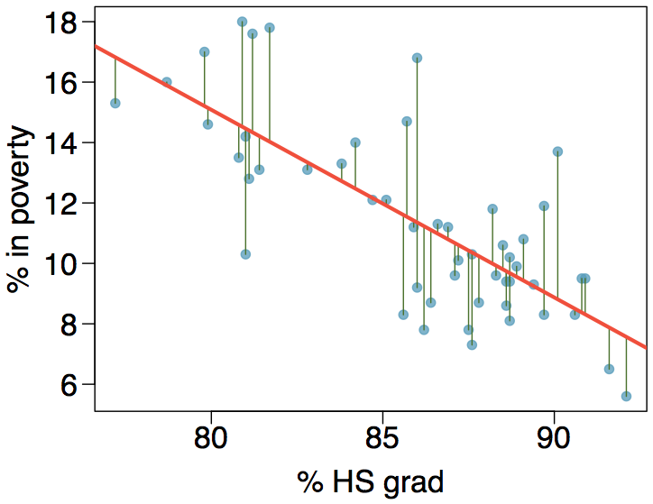
\includegraphics[width=0.75\textwidth,height=\textheight]{images/all_residuals.png}

\hypertarget{section-2}{%
\subsubsection{\texorpdfstring{\href{}{}}{}}\label{section-2}}

It would make sense then, that the \emph{best line} for any given
scatterplot, is the one that minimizes all of the residuals. This is the
idea behind \textbf{Least Squares Regression}, a method for finding that
best line. We won't get into the technical details of how least squares
regression works, but I want to cover just the basic concept:

\begin{itemize}
\item
  We consider many potential lines for the best line (each with
  different slope and intercept)

  \begin{itemize}
  \tightlist
  \item
    technology allows us to consider ALL potential lines at the same
    time
  \end{itemize}
\item
  We \textbf{square} all of the residuals for each line

  \begin{itemize}
  \tightlist
  \item
    residuals are squared so they all become positive, and so we can
    give a bigger `penalty' to points that are really far from the model
  \end{itemize}
\item
  The line that gives us the \textbf{smallest sum of all squared
  residuals} is our best model for the data.

  \begin{itemize}
  \tightlist
  \item
    hence the name, least squares regression
  \end{itemize}
\end{itemize}

I think there is a benefit to visualizing this process. Watch the video
below of me walking you through different lines for a dataset and see
the squared residuals change. Then you can follow the link provided to
play around yourself.

~

\begin{quote}
\href{https://dtkaplan.shinyapps.io/DA_least_squares/}{Visualize least
square regression}
\end{quote}

\hypertarget{estimating-the-equation}{%
\subsubsection{Estimating the Equation}\label{estimating-the-equation}}

\[\hat{y}=\beta_0+\beta_1\cdot x\]

This is our Least Squares Regression equation. We need to think about
the intercept and slope as \textbf{parameters} for us to estimate using
sample data. We estimate the intercept and slope with \(b_0\) and
\(b_1\) respectively. So the estimated regression equation is:

\[\hat{y}=b_0+b_1\cdot x\]

\hypertarget{section-3}{%
\subsubsection{\texorpdfstring{\href{}{}}{}}\label{section-3}}

For the most part, we will get these estimates using R, but there is a
simple way to find them with just the sample standard deviations and the
correlation coefficient. First we estimate the slope:

\[b_1=\frac{s_y}{s_x}\cdot R\]

And once we have that, we can find the intercept with the sample means
and slope estimate:

\[b_0=\bar{y}-b_1\cdot \bar{x}\]

\hypertarget{try-it-out}{%
\subsubsection{Try it out}\label{try-it-out}}

Give it a shot using the summary statistics below from the HS grad rate
and Poverty level example.

~

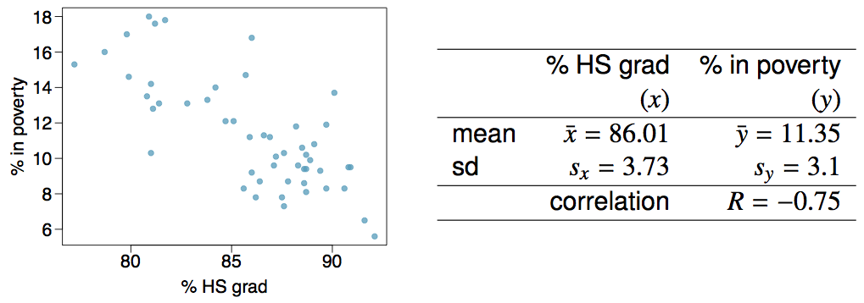
\includegraphics[width=0.85\textwidth,height=\textheight]{images/reg_example.png}

Use the code box below for calculations if you like What is the slope
estimate, \(b_1\), from the sample data?\footnote{c}

\begin{enumerate}
\def\labelenumi{\alph{enumi})}
\item
  1.28
\item
  -0.90
\item
  -0.62
\item
  0.83
\end{enumerate}

What is the intercept estimate, \(b_0\), from the sample data?\footnote{b}

\begin{enumerate}
\def\labelenumi{\alph{enumi})}
\item
  -41.97
\item
  64.68
\item
  -80.11
\item
  78.97
\end{enumerate}

\hypertarget{interpreting-slope-and-intercept}{%
\subsection{Interpreting Slope and
Intercept}\label{interpreting-slope-and-intercept}}

\hypertarget{section-4}{%
\subsubsection{\texorpdfstring{\href{}{}}{}}\label{section-4}}

One important thing to remember when writing or talking about your
regression equation (or any analysis) is to put context to the numbers.
\textbf{Your equation should never \emph{actually} use the letters \(y\)
and \(x\). And you should never give a generic interpretation of the
intercept and slope.}

I may use \(x\) and \(y\) in examples and to illustrate a point, but
when you're using real data, those are just letters that don't mean
anything. In the previous example, I would not accept a regression
equation like this:

\[\hat{y}=64.68-0.62\cdot x\]

I'd much rather have you write:

\[\hat{\text{% in poverty}}=64.68-0.62\cdot \text{% HS grad}\]

\hypertarget{slope-interpretation}{%
\subsubsection{Slope interpretation}\label{slope-interpretation}}

This is the big one, the one that explains the entire relationship
between the response and explanatory variables. This is the only time
you will see me give you a generic interpretation. For any dataset, fill
in the blue parts with the appropriate context.

\begin{quote}
For an increase of one unit in the explanatory variable, we can expect
that the response variable will change by the amount of the slope
coefficient value.
\end{quote}

Notice that the amount we increase \(x\) is not blue, meaning you should
always interpret the slope as the change in \(y\) for \textbf{one}
increase in \(x\). You can also make the interpretation sound a little
nicer than what I have up there, but it's a starting point.

Using the previous example. Select the best interpretation of the slope
coefficient, -0.62:\footnote{c}

\begin{enumerate}
\def\labelenumi{\alph{enumi})}
\item
  As x increases by 1, y changes by -0.62
\item
  As poverty increases by 1\%, we can expect the high school graduation
  rate to decrease by 0.62\%
\item
  As high school graduation increases by 1\%, we can expect the poverty
  rate to decrease by 0.62\%
\item
  As high school graduation increases by 1\%, we can expect the poverty
  rate to increase by 0.62\%
\end{enumerate}

\hypertarget{intercept-interpretation}{%
\subsubsection{Intercept
interpretation}\label{intercept-interpretation}}

Although typically less important for the understanding of the
relationship, we can still interpret the intercept. Once again, fill in
the blue text for the generic interpretation below with the data
context.

\begin{quote}
When the explanatory variable is zero, we can expect the response
variable to be equal to the intercept value.
\end{quote}

Notice that the intercept always describes \(y\), when \(x=0\). Also
take note that in real data, it will often not make much sense for the
explanatory variable to be zero. This leads to an intercept
interpretation that sounds like non-sense. It's fine, we do need the
intercept in order to define our line, but we don't need it to make
sense in the context of the problem.

Using the previous example. Select the best interpretation of the
intercept value, 64.68:\footnote{b}

\begin{enumerate}
\def\labelenumi{\alph{enumi})}
\item
  When \(x=0\), \(y=64.68\)
\item
  When the high school graduation rate is 0\% in a state, we can expect
  the poverty rate to be 64.68\%
\item
  When the poverty rate is 0\% in a state, we can expect the high school
  graduation rate to be 64.68\%
\item
  When the high school graduation rate is 64.68\%, we can expect the
  poverty rate to be 0\%
\end{enumerate}

Does the interpretation of the intercept make real world
sense?\footnote{c}

\begin{enumerate}
\def\labelenumi{\alph{enumi})}
\item
  No, not at all. The intercept is not even a possible value for poverty
  rate.
\item
  Yes, it makes perfect sense.
\item
  Not \emph{really}, while the intercept is possible for the poverty
  rate, it's not realistic for the high school graduation rate to be 0\%
  for a state. \#\#\# \href{}{}
\end{enumerate}

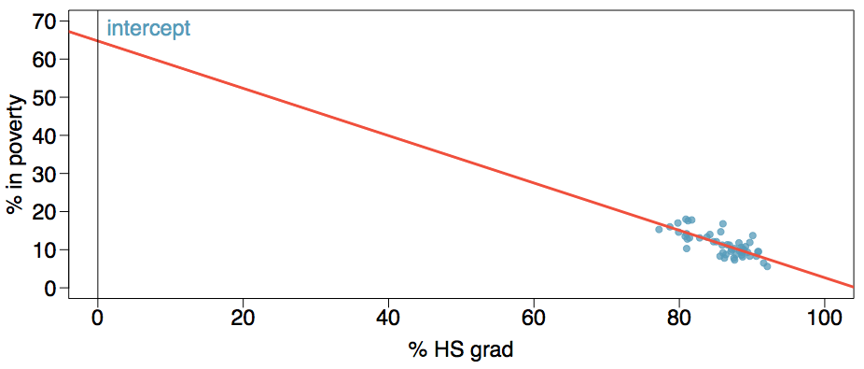
\includegraphics[width=0.85\textwidth,height=\textheight]{images/intercept.png}

\hypertarget{introducing-r2}{%
\subsection{\texorpdfstring{Introducing
\(R^2\)}{Introducing R\^{}2}}\label{introducing-r2}}

\hypertarget{section-5}{%
\subsubsection{\texorpdfstring{\href{}{}}{}}\label{section-5}}

We will talk about one more numeric statistic for understanding linear
regression models better, \(R^2\). Remember the correlation coefficient,
\(R\)? Well, \(R^2\) is just what you might expect, the correlation
squared. This means that \(R^2\) must be between 0 and 1.

\[R^2=(R)^2=correlation^2\]

This is a very useful statistic as a measure of the ``model fit'', or
how well the points in the scatterplot actually form a line. The
stronger the linear relationship \(\Rightarrow\) the closer the
correlation is to -1 or 1 \(\Rightarrow\) the closer \(R^2\) is to 1
\(\Rightarrow\) \textbf{the better the model fits the data}.

Another way to think bout \(R^2\) is as the proportion of variability in
the response variable that is explained by the linear model. Naturally,
we would like our model to explain as much variability as possible, so
we like it when \(R^2\) is closer to 1. Any leftover variability is just
unexplained and unknown.

Remember that the correlation from the previous example is \(R=-0.75\).
Calculate the \(R^2\) value.

Select the best interpretation of the \(R^2\) value.\footnote{b}

\begin{enumerate}
\def\labelenumi{\alph{enumi})}
\item
  38\% of the variability in the percent of HG graduates among the 51
  states is explained by the model.
\item
  38\% of the variability in the percent of residents living in poverty
  among the 51 states is explained by the model.
\item
  38\% of the time percent HS graduates predict percent living in
  poverty correctly.
\item
  62\% of the variability in the percent of residents living in poverty
  among the 51 states is explained by the model.
\end{enumerate}

\hypertarget{section-6}{%
\subsubsection{\texorpdfstring{\href{}{}}{}}\label{section-6}}

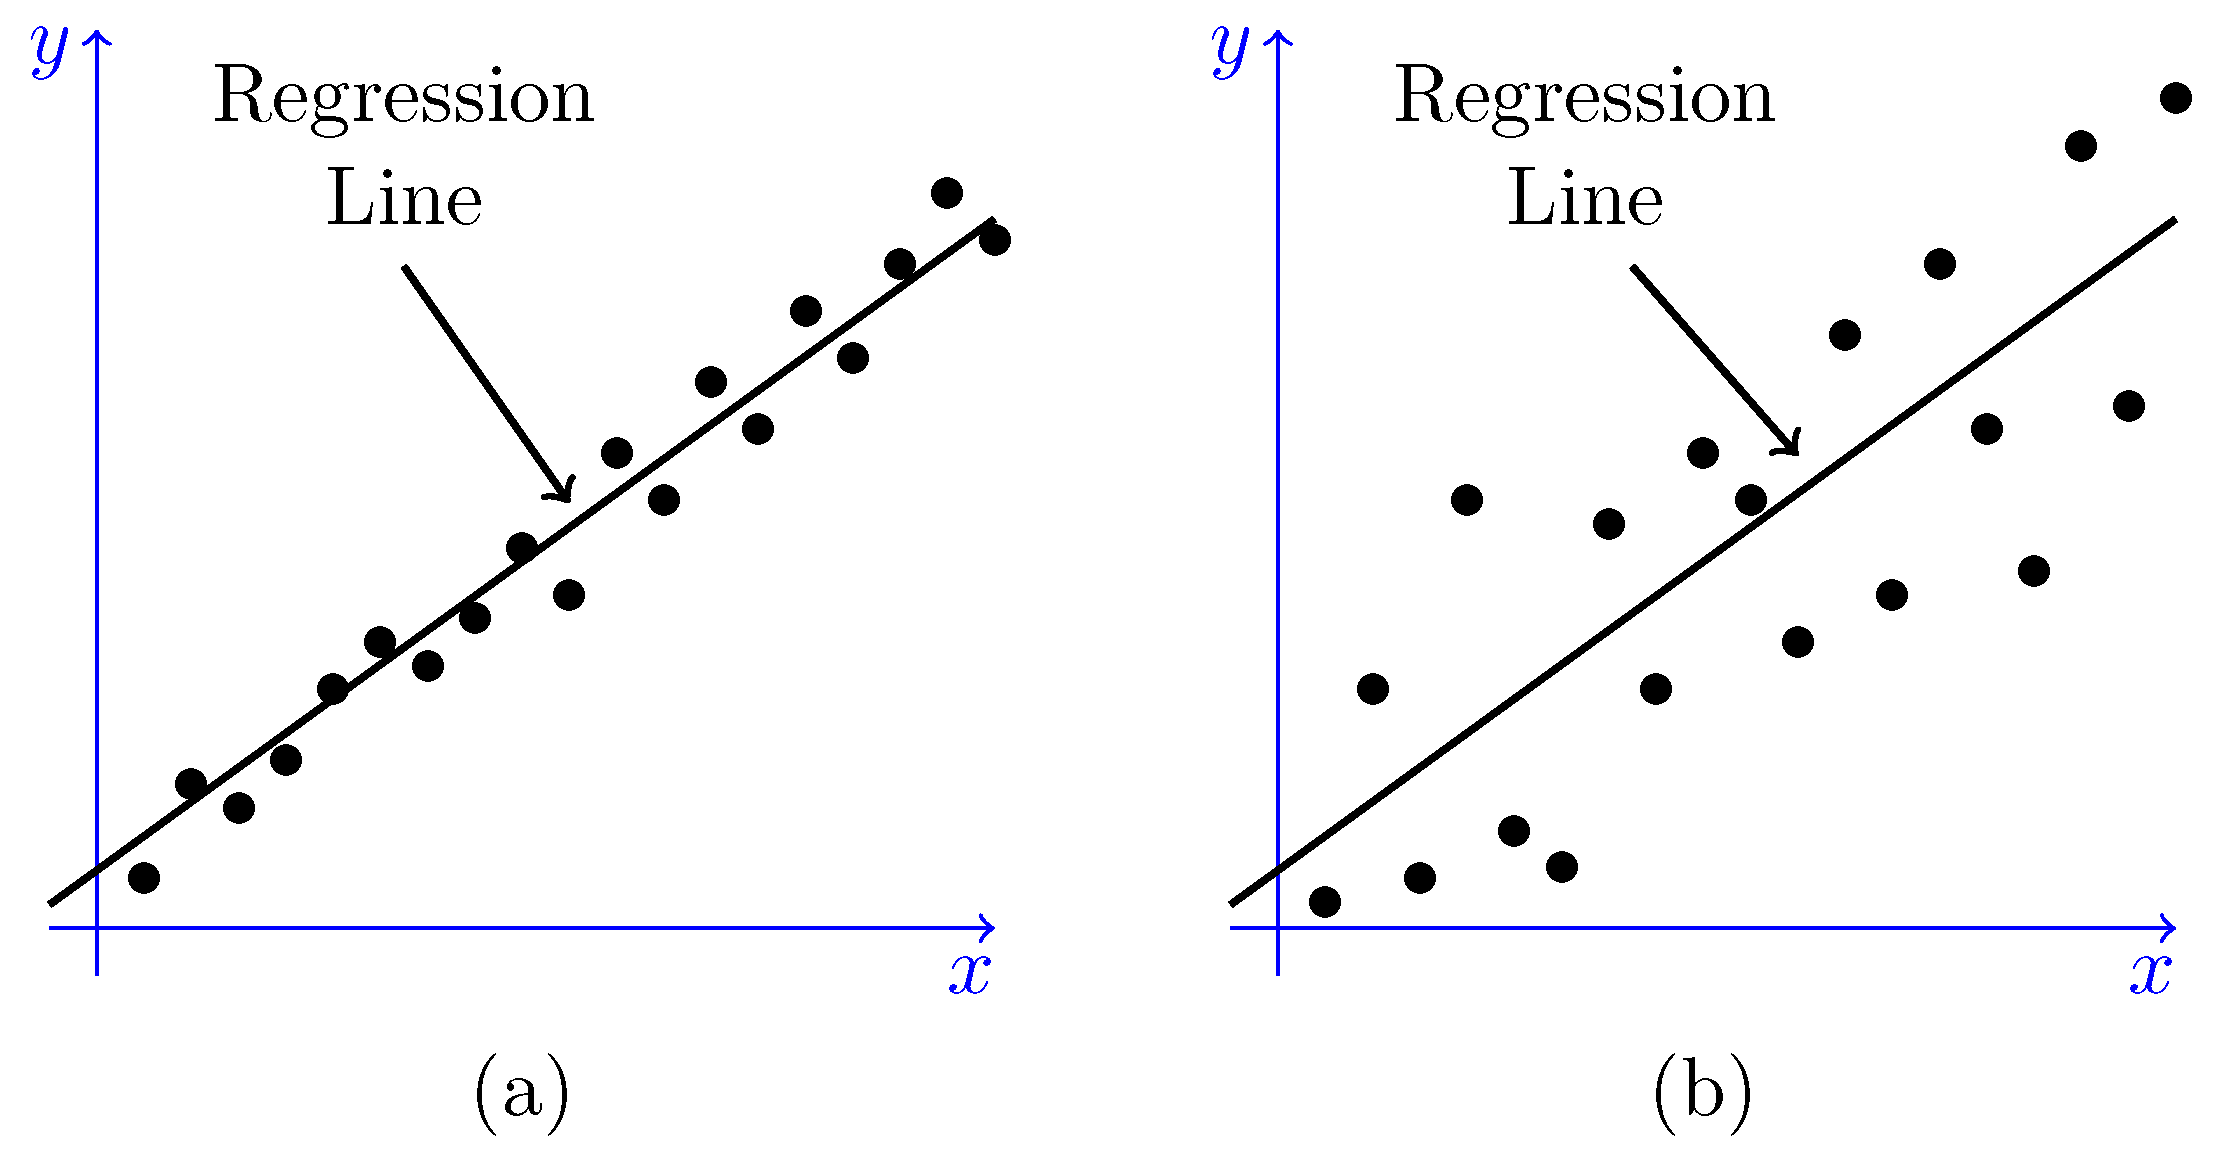
\includegraphics[width=0.75\textwidth,height=\textheight]{images/rsquare-color.png}

Which plot above would have the higher \(R^2\) value?\footnote{a}

\begin{enumerate}
\def\labelenumi{\alph{enumi})}
\item
  \begin{enumerate}
  \def\labelenumii{(\alph{enumii})}
  \item
  \end{enumerate}
\item
  \begin{enumerate}
  \def\labelenumii{(\alph{enumii})}
  \setcounter{enumii}{1}
  \item
  \end{enumerate}
\end{enumerate}

\hypertarget{section-7}{%
\subsubsection{\texorpdfstring{\href{}{}}{}}\label{section-7}}

\includegraphics[width=0.55\textwidth,height=\textheight]{https://imgs.xkcd.com/comics/linear_regression.png}

\hypertarget{using-the-model}{%
\subsection{Using the Model}\label{using-the-model}}

\hypertarget{interpreting-predictions}{%
\subsubsection{Interpreting
Predictions}\label{interpreting-predictions}}

Other than defining the relationship between response and explanatory,
the regression model is useful for making predictions. This is one of
the most interesting parts of linear regression, where you get to test
out your model and see how well it performs in the real world.

Take the previous example, if we know that the high school graduation
rate for 2016 (most currently available data) in Minnesota was 82.2\%,
what can we expect the poverty rate to be that year?

\(\hat{\text{% in poverty}}=64.68-.062\cdot \text{% HS grad}\)

What is the expected poverty rate for MN in 2016 if the HS grad rate was
82.2\%?\footnote{c}

\begin{enumerate}
\def\labelenumi{\alph{enumi})}
\item
  10.8\%
\item
  64.68\%
\item
  13.72\%
\item
  115.64\%
\end{enumerate}

\hypertarget{beware}{%
\subsubsection{BEWARE!}\label{beware}}

While predictions are fun and interesting, you need to be mindful about
making predictions beyond the information you have. \textbf{Never make a
prediction using a value of the explanatory variable outside the range
of values that was observed}. This is a major risk and is called
\textbf{Extrapolation}.

\begin{quote}
The relationship in the \emph{observed} data may be linear, you there is
no guarantee that the linear pattern extends \emph{before or after what
was observed}.
\end{quote}

What is the average age of men's first marriage would you predict for
1960 using this data? 1990? 2020?

~

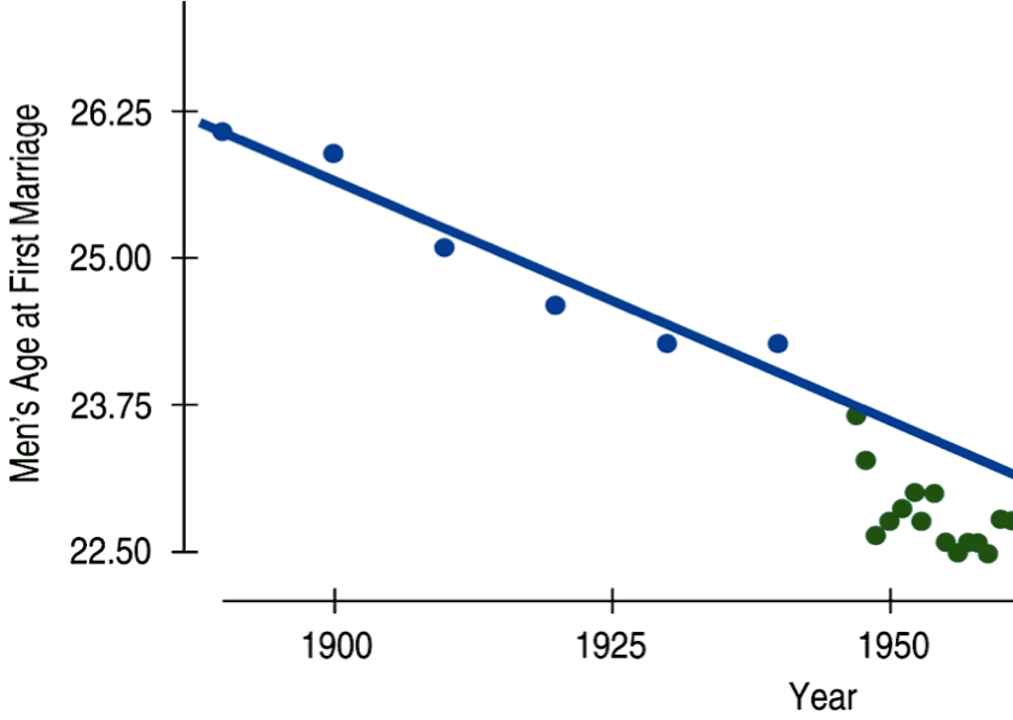
\includegraphics[width=0.65\textwidth,height=\textheight]{images/extrap_before.png}

\hypertarget{section-8}{%
\subsubsection{\texorpdfstring{\href{}{}}{}}\label{section-8}}

Be careful not to extrapolate the model and make predictions past what
was observed. This is especially true when dealing with time as an
explanatory variable. Trends change and cycle, we wouldn't expect the
pattern to stay as a negative relationship or else average age at first
marriage would eventually be 0 or even negative!

~

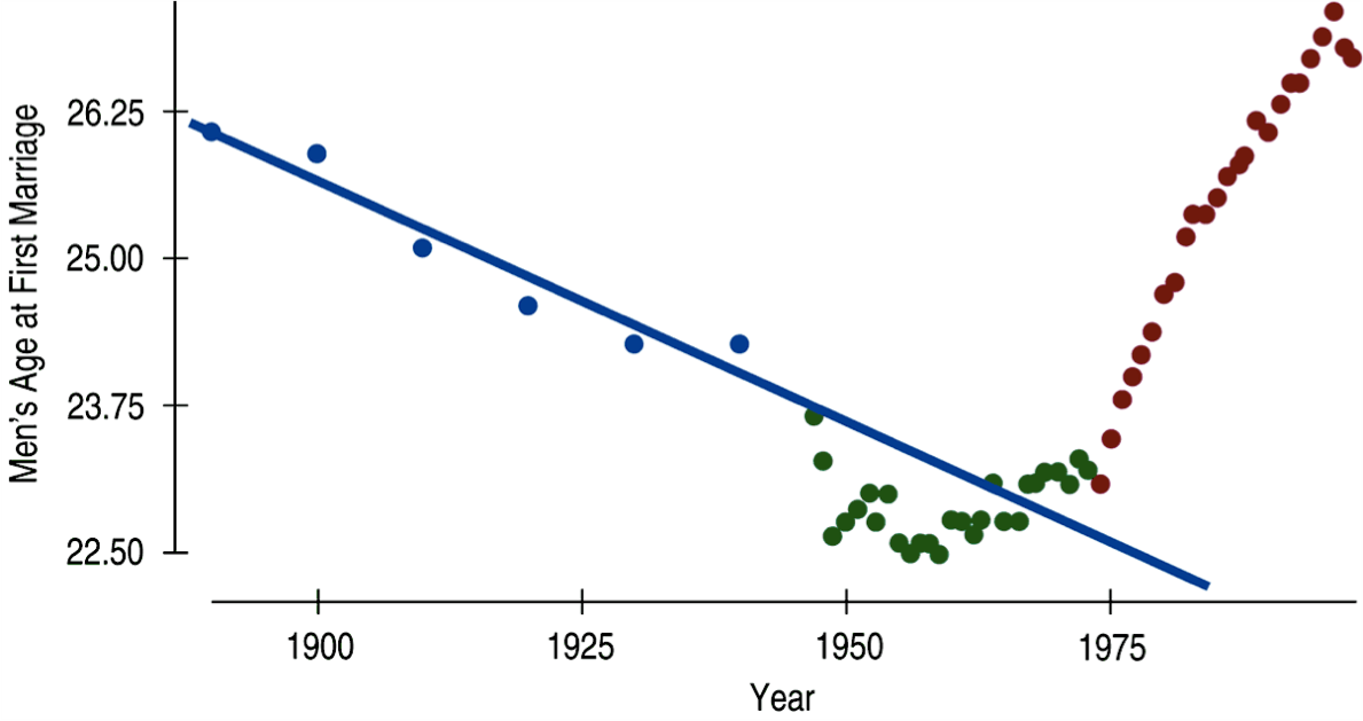
\includegraphics[width=0.85\textwidth,height=\textheight]{images/extrap_after.png}

\hypertarget{example-in-r}{%
\subsection{Example in R}\label{example-in-r}}

\hypertarget{used-car-prices}{%
\subsubsection{Used car prices}\label{used-car-prices}}

Can you predict the price of a used Porsche by only using the mileage?
The data below contains the price and mileage of 30 used Porsches. Note
that the \texttt{Price} is measured in thousands of dollars and
\texttt{Mileage} is measured in thousands of miles.

~

\begin{Shaded}
\begin{Highlighting}[]
\NormalTok{porsche <-}\StringTok{ }\KeywordTok{read.csv}\NormalTok{(}\StringTok{"~/Stats 212b S20/Class/Data/PorschePrice.csv"}\NormalTok{)}
\end{Highlighting}
\end{Shaded}

~

\begin{verbatim}
##    Price Age Mileage
## 1   69.4   3   21.50
## 2   56.9   3   43.00
## 3   49.9   2   19.90
## 4   47.4   4   36.00
## 5   42.9   4   44.00
## 6   36.9   6   49.80
## 7   83.0   0    1.30
## 8   72.9   0    0.67
## 9   69.9   2   13.40
## 10  67.9   0    9.70
## 11  66.5   2   15.30
## 12  64.9   2    9.50
## 13  58.9   4   19.10
## 14  57.9   3   12.90
## 15  54.9  10   33.90
## 16  54.7  11   26.00
## 17  53.7   4   20.40
## 18  51.9   4   27.50
## 19  51.9  10   51.70
## 20  49.9   3   32.40
## 21  44.9   4   44.10
## 22  44.8  13   49.80
## 23  39.9   6   35.00
## 24  39.7   6   20.50
## 25  34.9   8   62.00
## 26  33.9   7   50.40
## 27  23.9  20   89.60
## 28  22.9  22   83.40
## 29  16.0  20   86.00
## 30  52.9   3   37.40
\end{verbatim}

~

Set up the variables. What is the response variable?\footnote{a}

\begin{enumerate}
\def\labelenumi{\alph{enumi})}
\item
  Price
\item
  Mileage
\item
  Age
\end{enumerate}

What is the explanatory variable?\footnote{b}

\begin{enumerate}
\def\labelenumi{\alph{enumi})}
\item
  Price
\item
  Mileage
\item
  Age
\end{enumerate}

\hypertarget{eda-summarize-and-visualize}{%
\subsubsection{EDA: Summarize and
visualize}\label{eda-summarize-and-visualize}}

Plot the variables and find the correlation coefficient. Plug in the
appropriate variables in the code.

The correlation coefficient \emph{suggests} that the relationships
are:\footnote{a,c,e}

\begin{enumerate}
\def\labelenumi{\alph{enumi})}
\item
  linear
\item
  non-linear
\item
  negative
\item
  positive
\item
  strong
\item
  moderate
\item
  weak
\end{enumerate}

\hypertarget{find-the-line}{%
\subsubsection{Find the line}\label{find-the-line}}

What is the best line to describe the relationship between
\texttt{Price} and \texttt{Mileage}? Use \texttt{lm()} (for `linear
model'), this function uses arguments in the
\texttt{Response\ \textasciitilde{}\ Explanatory,\ data\ =\ dataset\_name}
form.

Just like we did for ANOVA, we will want to save the model as a named
object in R so we can refer to it later and pull out more information.
You can use any name for your model. Try to fit the linear regression
line and get the slope and intercept estimates for the Porsche data.

\begin{verbatim}
## 
## Call:
## lm(formula = Price ~ Mileage, data = porsche)
## 
## Residuals:
##      Min       1Q   Median       3Q      Max 
## -19.3077  -4.0470  -0.3945   3.8374  12.6758 
## 
## Coefficients:
##             Estimate Std. Error t value Pr(>|t|)    
## (Intercept) 71.09045    2.36986    30.0  < 2e-16 ***
## Mileage     -0.58940    0.05665   -10.4 3.98e-11 ***
## ---
## Signif. codes:  0 '***' 0.001 '**' 0.01 '*' 0.05 '.' 0.1 ' ' 1
## 
## Residual standard error: 7.17 on 28 degrees of freedom
## Multiple R-squared:  0.7945, Adjusted R-squared:  0.7872 
## F-statistic: 108.3 on 1 and 28 DF,  p-value: 3.982e-11
\end{verbatim}

What is the equation of the regression line?\footnote{b}

\begin{enumerate}
\def\labelenumi{\alph{enumi})}
\item
  \(\hat{y}=\beta_0+\beta_1\cdot x\)
\item
  \(\hat{\text{Price}}=71.1-0.59\cdot \text{Mileage}\)
\item
  \(\hat{\text{Price}}=-0.59+71.1\cdot \text{Mileage}\)
\item
  \(\hat{\text{Price}}=2.37+0.057\cdot \text{Mileage}\)
\end{enumerate}

\hypertarget{section-9}{%
\subsubsection{\texorpdfstring{\href{}{}}{}}\label{section-9}}

There are plenty of different ways to make scatterplots and add the
regression line, but I think this is one of the simplest. (Be sure you
load the \texttt{mosaic} package before using any \texttt{gf\_}
functions.)

\includegraphics{Regression_line_hardcopy_files/figure-latex/plot-1.pdf}

\hypertarget{interpret-the-values}{%
\subsubsection{Interpret the values}\label{interpret-the-values}}

\[\hat{\text{Price}}=71.1-0.59\cdot \text{Mileage}\]

Think about how you would interpret the intercept and slope. Do they
make sense in the context of the problem?

How would you interpret the slope coefficient?\footnote{b}

\begin{enumerate}
\def\labelenumi{\alph{enumi})}
\item
  For every extra one mile on a used Porsche, the expected price will
  decrease by 59 cents.
\item
  For every extra one thousand miles on a used Porsche, the expected
  price will decrease by \$590.
\item
  For every extra 590 miles on a used Porsche, the expected price will
  decrease by \$71,100.
\item
  For every extra 590 miles on a used Porsche, the expected Price will
  decrease by \$1,000.
\end{enumerate}

How would you interpret the intercept value?\footnote{a}

\begin{enumerate}
\def\labelenumi{\alph{enumi})}
\item
  For a used Porsche that has zero miles on it, we would expect an
  average asking price of \$71,100.
\item
  For a used Porsche with 71,100 miles on it, we would expect an average
  asking price of \$0.
\item
  For a used Porsche with 0 miles on it, we would expect an average
  asking price of \$71.10.
\item
  For a used Porsche with 71.1 miles on it, we would expect an average
  asking price of -\$590.
\end{enumerate}

Does the intercept interpretation make sense for this data?\footnote{a}

\begin{enumerate}
\def\labelenumi{\alph{enumi})}
\item
  Yes, it does.
\item
  No, it does not.
\end{enumerate}

Look back at the \texttt{R} output summary of the regression model for
the \(R^2\) value and select the best interpretation. (The code is in
the second \texttt{Hint} in the \emph{Find the line} section if you need
help getting the summary. You can use the
\texttt{Adjusted\ R-squared})\footnote{c}

\begin{enumerate}
\def\labelenumi{\alph{enumi})}
\item
  This model will accurately predict the price of 78\% of all used
  Porsches.
\item
  On average, the price of our predictions using the model is off by
  \$78.72.
\item
  Our model, using mileage, is able to predict 78\% of the variation we
  see in the price of used Porsches.
\item
  78\% of the points on the scatterplot are close to the line.
\end{enumerate}

\hypertarget{make-a-couple-predictions}{%
\subsubsection{Make a couple
predictions}\label{make-a-couple-predictions}}

\[\hat{\text{Price}}=71.1-0.59\cdot \text{Mileage}\]

I'm in the market for a used Porsche (OK, not really), and I found a few
different options. What should sort of offers should I make on the
following cars? Use the code box for calculations if you'd like.

What should I offer for a car I found that has 60,000 miles on
it?\footnote{d}

\begin{enumerate}
\def\labelenumi{\alph{enumi})}
\item
  \$4,265.41
\item
  -\$35,328.90
\item
  \$35.70
\item
  \$35,700
\item
  Don't use this model to make an offer.
\end{enumerate}

What should I offer for a car that has 150,000 miles on it?\footnote{a}

\begin{enumerate}
\def\labelenumi{\alph{enumi})}
\item
  Don't use this model to make an offer.
\item
  \$17,400
\item
  -\$17,400
\item
  -\$17.40
\end{enumerate}

If I had a budget of \$20,000 for buying my used Porsche, about what
mileage should I being looking at?\footnote{b}

\begin{enumerate}
\def\labelenumi{\alph{enumi})}
\item
  Around 59,000 miles
\item
  Around 86,000 miles
\item
  Around 86 miles
\item
  Around 59 miles
\item
  Impossible to determine``, message =''Plug in 20 as the price in the
  model and work backwards to solve for the mileage.
\end{enumerate}

I found a car with 65,000 miles on it and the owner was asking \$29,000.
What is the residual for this observation and should I take the deal or
negotiate?\footnote{a}

\begin{enumerate}
\def\labelenumi{\alph{enumi})}
\item
  The residual is -\$3,750, I should take the deal.``, correct = TRUE,
  message =''A negative residual means the model \textbf{overestimated}
  the price.
\item
  The residual is -\$3,750, I should negotiate a better price.``,
  message =''This is the correct residual, but the asking price is less
  than what the model predicts, so I'd probably be better off taking the
  deal.
\item
  The residual is \$3,750, I should take the deal.
\item
  The residual is \$3,750, I should negotiate a better deal.
\end{enumerate}

\hypertarget{bonus-time}{%
\subsection{Bonus Time}\label{bonus-time}}

Feel free to create a linear regression model for the relationship
between \texttt{Price} and \texttt{Age} of used Porsches, or
\texttt{Age} and \texttt{Mileage}. I think for this particular dataset
you could create a reasonable research question where any variable is
the response or explanatory. Play around and get some practice.


\end{document}
